\documentclass[11pt]{article}
\usepackage{nodalida2017}
\usepackage{amsmath}
\usepackage{enumitem}
\usepackage{mathptmx}
\usepackage{xcolor}
\usepackage{graphicx}
\usepackage{url}
\usepackage{latexsym}
\usepackage{fancyvrb}

\title{Exploring the Expressivity of Constraint Grammar}

\author{%
  Wen Kokke \\
  University of Edinburgh \\
  {\tt wen.kokke@ed.ac.uk} \\\And
  Inari Listenmaa \\
  University of Gothenburg \\
  {\tt inari.listenmaa@cse.gu.se} }

\date{\today}

\def\t#1{\texttt{#1}}
\def\h#1{{\tt \color{gray} #1}}
\def\swf{\h{"<s>"}}
\def\maxAmb#1{$\langle \Sigma \rangle_#1$}
\def\maxAmbFSA#1{$\langle \Sigma,S \rangle_#1$}
\def\maxAmbCFG#1{$\langle \Sigma,\Sigma^{\prime} \rangle_#1$}
\def\exampleWord{{\color{red} TODO}}

\begin{document}
\maketitle

\begin{abstract}
  We believe that for any formalism which has its roots in linguistics, it is a
  natural question to ask ``how expressive is it?'' Therefore, in this paper, we
  begin to address the question of the expressivity of CG.
  Aside from the obvious theoretical interest, we envision also practical
  benefits. For instance, we hope that the FSA$\rightarrow$CG conversion tool, described in
  later sections of this paper, could eventually be developed to generate
  human-readable CG code from regular expressions or a context-free grammar. 
\end{abstract}


\section{Introduction}
For any formalism with its root in linguistics, it is natural to ask questions
such as ``How expressive is it?'' or ``Where does it sit in the Chomsky
hierarchy?''~\cite{chomsky1956hierarchy}
In this paper, we begin addressing some of these questions for constraint
grammar~\cite[CG]{karlsson1995constraint}.

Before we can even consider such a question, there is a problem we must
solve. CG was never meant to be a grammar in the generative sense. Instead, it
is a tool for analysing and disambiguating strings.
This, we believe, explains why the question of the expressivity of CG went
unasked and unanswered for a long time.
It also gives us our first problem: How do we view CGs generatively?
We address this in section~\ref{sec:gencg}.


\section{Generative Constraint Grammar}\label{sec:gencg}
We view a constraint grammar CG as generating a formal language $\mathcal{L}$
over an alphabet $\Sigma$ as follows.
We encode words $w \in \Sigma^\star$ as a sequence of cohorts, each of which has
one of the symbols of $w$ as a reading.
A constraint grammar CG rejects a word if, when we pass its encoding through the
CG, we get back the cohort \t{"<REJECT>"}. A constraint grammar CG accepts a word
if it does not reject it.
We generate the language $\mathcal{L}$ by passing every $w \in \Sigma^\star$
through the CG, and keeping those which are accepted.

As an example, consider the language $a^\star$ over $\Sigma = \{a,b\}$.
This language is encoded by the following constraint grammar:
\begin{center}
  \begin{Verbatim}
    LIST A = "a";
    LIST B = "b";
    SET LETTER = A OR B;
    SELECT A;
    ADDCOHORT ("<REJECT>")
        BEFORE LETTER 
        IF (-1 (>>>) LINK 1* B);
    REMCOHORT LETTER
        IF (-1* ("<REJECT>"));
  \end{Verbatim}
\end{center}
We then encode the input words as a series of letter cohorts with readings
(e.g.\ \(\t{"<l>"}\;\t{"a"}\), \(\t{"<l>"}\;\t{"b"}\)), and run the grammar.
For instance, if we wished to know whether either word in $\{aaa,aab\}$ is part
of the language $a^\star$, we would run the following queries:
\begin{center}
  \begin{tabular}{l|c}
    \textbf{Input}         & \textbf{Output} \\ \hline
    \(\t{"<l>"}\;\t{"a"}\) & \(\t{"<l>"}\;\t{"a"}\) \\
    \(\t{"<l>"}\;\t{"a"}\) & \(\t{"<l>"}\;\t{"a"}\) \\
    \(\t{"<l>"}\;\t{"a"}\) & \(\t{"<l>"}\;\t{"a"}\) \\ \hline
    \(\t{"<l>"}\;\t{"a"}\) & \t{"<REJECT>"} \\
    \(\t{"<l>"}\;\t{"a"}\) \\
    \(\t{"<l>"}\;\t{"b"}\)
  \end{tabular}
\end{center}
As CG is a tool meant for disambiguation, we can leverage its power to run both
queries at once:
\begin{center}
  \begin{tabular}{l|c}
    \textbf{Input}                  & \textbf{Output} \\ \hline
    \(\t{"<l>"}\;\t{"a"}\)          & \(\t{"<l>"}\;\t{"a"}\) \\
    \(\t{"<l>"}\;\t{"a"}\)          & \(\t{"<l>"}\;\t{"a"}\) \\
    \(\t{"<l>"}\;\t{"a"}\;\t{"b"}\) & \(\t{"<l>"}\;\t{"a"}\)
  \end{tabular}
\end{center}
This is a powerful feature, because it allows us disambiguate based on some
formal language $\mathcal{L}$ if we can find the CG which generates it.
However, the limitations of this style become apparent when we look at a run of
a CG for the language $\{ab,ba\}$:
\begin{center}
  \begin{tabular}{l|c}
    \textbf{Input}                  & \textbf{Output} \\ \hline
    \(\t{"<l>"}\;\t{"a"}\;\t{"b"}\) & \(\t{"<l>"}\;\t{"a"}\;\t{"b"}\) \\
    \(\t{"<l>"}\;\t{"a"}\;\t{"b"}\) & \(\t{"<l>"}\;\t{"a"}\;\t{"b"}\) \\
  \end{tabular}
\end{center}
While the output contains the interpretations $ab$ and $ba$, it also includes
$aa$ and $bb$. Therefore, while this style is useful for disambiguating using
CGs based on formal languages, it is too limited to be used in defining the
language which a CG generates.
% Wen:
%   We should include a reference to the other formalism here, or to the
%   discussion section in which we talk about the disjunction problem.
% Inari:
%   Yeah, I am wondering myself too what's the best place to talk about it.
%   Maybe it becomes easier when we have more pages to fill? 

In light of the idea of using CGs based on formal languages for disambiguating,
it seems at odds with the philosophy of CG to reject by replacing the entire
input with a single \t{"<REJECT>"} cohort. CG generally refuses to remove the
last possible reading of a cohort, under the philosophy that \emph{some}
information is certainly better than none.
However, for the definition of CG as a formal language, we need some sort of
distinctive output for rejections. Hence, we arrive at \emph{two} distinct ways
to run generative CGs: the method in which we input unambiguous strings, and
output \t{"<REJECT>"}, which is used in the definition of CG as a formal
language; and the method in which we input ambiguous strings, and simply
disambiguate as far as possible. 

It should be noted that VISL CG-3 \cite{bick2015,vislcg3} supports commands 
such as \t{EXTERNAL}, which runs an external executable. It should therefore 
be obvious that the complete set of VISL CG-3 commands, at least theoretically,
can generate any recursively enumerable language. For this reason, we will
investigate particular subsets of the commands permitted by CG.
In sections~\ref{sec:lowerbound} and~\ref{sec:regular}, we will restrict
ourselves to the subset of CG which only uses the \t{REMOVE} command with
sections, and show this to at least cover all regular languages and some
context-free and context-sensitive languages.
In section~\ref{sec:turingcomplete}, we will restrict ourselves to thesubset of
CG which only uses the \t{ADDCOHORT} and \t{REMCOHORT} commands with sections,
and show this to be Turing complete.

\section{A lower bound for CG}\label{sec:lowerbound}
In this section, we will only use the \t{REMOVE} command with sections, in
addition to a single use of the \t{ADDCOHORT} command to add the special cohort
\t{"<REJECT>"}, and a single use of the \t{REMCOHORT} command to clean up
afterwards. 
We show that, using only these commands, CG is capable of generating some
context-free and context-sensitive languages, which establishes a lower bound on 
the expressivity of CG (see Figure~\ref{fig:nocorr}).
%
\begin{figure}[h]
  \centering
  % Wen: This graphic needs to be updated, because you literally prove in the
  % next section that we cover all regular languages.
  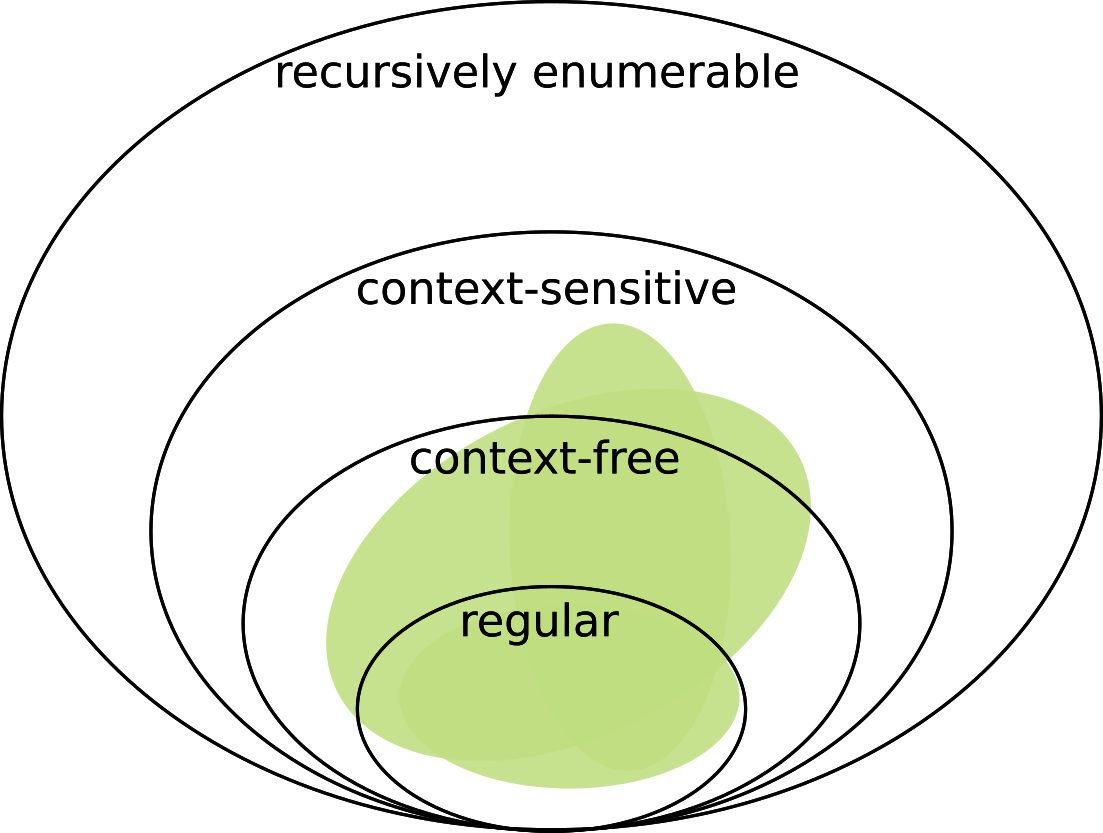
\includegraphics[width=0.8\linewidth]{chomsky}
  \caption{Lower bound on the expressivity of the subset of CG using only \t{REMOVE}.}
  \label{fig:nocorr}
\end{figure}


\subsection{Example grammar: $a^nb^n$}
Below, we briefly describe the CG which generates the language $a^nb^n$.
This CG is defined over the alphabet $\Sigma$, in addition to a hidden alphabet
$\Sigma^\prime$. These hidden symbols are meant to serve as a simple form of
memory. When we encode our input words, we tag each cohort with \emph{every}
symbol in the hidden alphabet\footnote{
  We can automatically add these hidden symbols to our cohorts using a single
  application of the \t{ADD} command.
}, e.g.\ for some symbol $\ell \in \Sigma$ and $\Sigma' = \{h_1,\dots,h_n\}$ we
would create the cohort \(\t{"<\(\ell\)>"}\;\t{"h\(_1\)"}\;\dots\;\t{"h\(_n\)"}\).

The CG for $a^nb^n$ uses the hidden alphabet \{\t{odd}, \t{even}, \t{opt\_a},
\t{opt\_b}\}. These symbols mean that the cohort they are attached to is in an
even or odd position, and that $a$ or $b$ is a legal option for this cohort,
respectively. The CG operates as follows: 
\begin{enumerate}
\item
  Is the number of characters even? We know the first cohort is odd, and the
  rest is handled with rules of the form \t{REMOVE even IF (NOT -1 odd)}. If the
  last cohort is odd, then discard the sentence. Otherwise continue\dots
\item
  The first cohort is certainly $a$ and last is certainly $b$, so we can
  disambiguate the edges: 
  \t{REMOVE opt\_b IF (NOT -1 (*))}, and \t{REMOVE opt\_a IF (NOT 1 (*))}. 
\item
  Disambiguate the second cohort as $a$ and second-to-last as $b$, the third as
  $a$ and third-to-last as $b$, etc, until the two ends meet in the middle. If
  every \t{"<a>"} is marked with \t{opt\_a}, and every \t{"<b>"} with
  \t{opt\_b}, we accept. Otherwise, we reject.  
\end{enumerate}
The language $a^nb^n$ is context-free, and therefore CG must at least partly
overlap with the context-free languages.


\subsection{Example grammar: $a^nb^nc^n$}
We can extend the approach used in the previous grammar to write a grammar which
accepts $a^nb^nc^n$. Essentially, we can adapt the above grammar to find the
middle of any input string. Once we have the middle, we can ``grow'' $a$s from
the top and $b$s up from the middle, and $b$s down from the middle and $c$s up
from the bottom, until we divide the input into three even chunks.
If this ends with all \t{"<a>"}s marked with \t{opt\_a}, all \t{"<b>"}s marked
with \t{opt\_b}, and all \t{"<c>"}s marked with \t{opt\_c}, we accept.
Otherwise, we reject.

The language $a^nb^nc^n$ is context-sensitive, and therefore CG must at least
partly overlap with the context-sensitive languages. 
%
\begin{figure}[t]
  \centering
  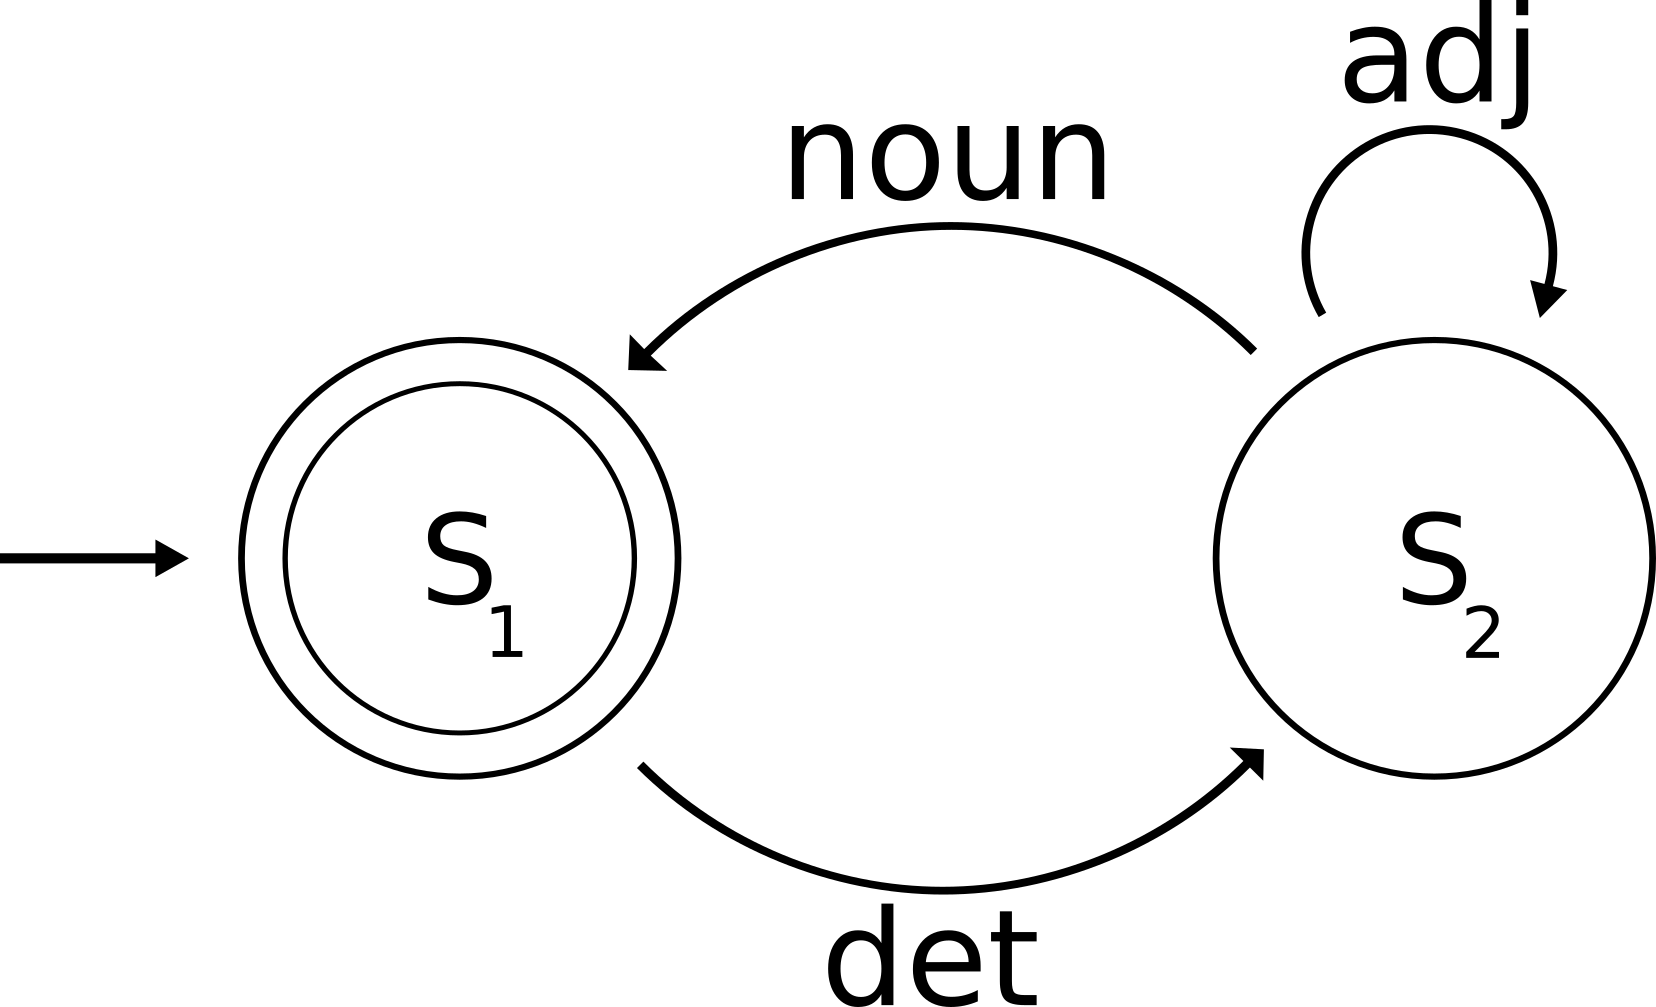
\includegraphics[width=0.6\linewidth]{fsa.png}
  \caption{A finite-state automaton describing the regular language \t{det
      (adj)* n}.}
 \label{fig:fsa}
\end{figure}


\section{Are all regular languages in CG?}\label{sec:regular}
In the present section, we propose a method to transform all regular
languages into CG. We show how any finite-state automaton can
be expressed in a CG: start with states and transitions as ambiguous
cohorts, and the disambiguated result shows both the correct sequence
and its path in the automaton.

\subsection{Finite-state automata}
Formally, a finite-state automaton is a 5-tuple
\[
  \langle \Sigma, S, s_0, \delta, F \rangle.
\]


$\Sigma$ is the alphabet of the automaton, $S$ is a set of states,
including a starting state $s_0$ and a set $F$ of final states.
$\delta$ is a transition function, which takes one state and one
symbol from the alphabet, and returns the state(s) where we can get
from the original state with that symbol.
The automaton in Figure~\ref{fig:fsa} is presented as follows:

\[\!
\begin{aligned}
  &S&      \!\!\!\!=\;& \{\t{S1}, \t{S2}\}   &&\Sigma& \!\!\!\!=\;& \{\emph{det, adj, n}\} \\
  &s_0&    \!\!\!\!=\;& \t{s1}               &&\delta&  \!\!\!\!=\;& \{\t{s1} \times \emph{det} = \{\t{s2}\}, \; \dots \}  \\ 
  &F&      \!\!\!\!=\;& \{\t{s1}\}           &&      & & %& \!\!\!\!  \;& \t{s2}   \times \emph{adj} = \t{s2}, ...
\end{aligned}
\]

Informally, the automaton describes a simple set of possible noun
phrases: there must be one determiner, one noun, and 0 or more
adjectives in between. 
We implement a corresponding CG in the following sections.

\subsection{Cohorts and sentences}

We encode our input as a sequence of \emph{state cohorts} and \emph{transition cohorts}.
Initially, a state cohort contains the full set $S = \{s_1, s_2\}$, and a
transition cohort contains $\Sigma = \{\emph{det, adj, n}\}$ or some
subset of it.
As an example, we generate all 2-letter words for the automaton in Figure~\ref{fig:fsa}.
The initial maximally ambiguous input for length 2 looks as follows:
%
\begin{center}
  \renewcommand{\tabcolsep}{2.5pt}
  \begin{tabular}{ccccc}
    \swf   & \t{"<w>"}  & \swf   & \t{"<w>"} & \swf   \\ 
    \h{s1} & \t{det}      & \h{s1} & \t{det} & \h{s1} \\
    \h{s2} & \t{adj}      & \h{s2} & \t{adj} & \h{s2} \\
           & \t{n}        &        & \t{n}   &               
  \end{tabular}
\end{center}
%
\noindent 
The rules of the grammar disambiguate both transition cohorts and state cohorts. Thus
the desired result shows both the accepted sequence, \emph{det n}, and the path in the automaton.
%
\begin{center}
  \renewcommand{\tabcolsep}{2.5pt}
  \begin{tabular}{ccccc}
    \swf   & \t{"<w>"}  & \swf   & \t{"<w>"} & \swf   \\ 
    \h{s1} & \t{det}    & \h{s2} & \t{n}     & \h{s1}       
  \end{tabular}
\end{center}
%
We can easily adapt the disambiguation scheme for real-world
ambiguities, such as ``the \exampleWord{}''\footnote{Choose whichever: the present,
  the sweet, ...}. The state cohorts are identical, but the transition
cohorts contain now some actual word form, and the initial ambiguity
is not over the whole $\Sigma$, but some subset of it.
%
\begin{center}
  \renewcommand{\tabcolsep}{2.5pt}
  \begin{tabular}{ccccc}
    \swf   & \t{"<the>"}  & \swf   & \t{"<\exampleWord{}>"} & \swf    \\ 
    \h{s1} & \t{det}      & \h{s1} & \t{adj}   & \h{s1}  \\
    \h{s2} &              & \h{s2} & \t{n}     & \h{s2}     
  \end{tabular}
\end{center}
%
The disambiguation process goes exactly like in the first version, with full
$\Sigma$ in the transition cohorts.
Depending on how much the initial input contains ambiguity, the
result may be the same, or more disambiguated. For our example, the
output is identical:
\begin{center}
  \renewcommand{\tabcolsep}{2.5pt}
  \begin{tabular}{ccccc}
    \swf   & \t{"<the>"}  & \swf   & \t{"<\exampleWord{}>"} & \swf    \\ 
    \h{s1} & \t{det}      & \h{s2} & \t{n}   & \h{s1}  \\
  \end{tabular}
\end{center}
%
%
\subsection{Rules}
Given that every transition happens between two states, and every state 
has an incoming and outgoing transition, every rule needs only
positions -1 and 1 in its contextual tests. 
The semantics of the rules are ``remove a reading (transition), if it is 
\emph{not} surrounded by allowed states'',
and ``remove a state, if it is \emph{not} surrounded by allowed transitions''.
For the example automaton, the POS-rules are as follows:
\begin{verbatim}
REMOVE...
  det IF (NEGATE -1 S1 LINK 2 S2);
  adj IF (NEGATE -1 S2 LINK 2 S2);
  n   IF (NEGATE -1 S2 LINK 2 S1);
\end{verbatim}
The start and end states naturally correspond to the first and last
state cohort, and can be trivially disambiguated, in this case both into \t{s1}.
Once we remove a reading from either side of a cohort, some more rules can take
action---the context ``\t{s2} on the left side and \t{s1} on the right side''
may be broken by removing either \t{s2} or \t{s1}. 

\subsection{Result}

For the final result of the disambiguation, we consider the two options.
In the first case, every cohort contains the whole alphabet,
and in the second case, only a subset.

\paragraph{Full $\Sigma$}
If there is only one allowed word of length $n$ in the language,
then the result will contain only fully disambiguated transition
cohorts.
Furthermore, if there is only path in the automaton that leads
to this word, then also the state cohorts are fully disambiguated.

If there are multiple strings of the same length in the language, then
we have to relax our criteria: every transition cohort in the result
may contain multiple readings, but all of them must contribute to some
valid word of length $n$.
If there are multiple paths in the automaton to reach the accepted
word(s), then the state cohorts may also be ambiguous.

\paragraph{Subset of $\Sigma$}
If the initial input is malformed, for example, ``the \exampleWord''
is missing a \t{det} reading in the first transition cohort, then the
output will be incorrect.

If the initial input is well-formed, then the result may be
disambiguated further than with the full $\Sigma$ in the transition cohorts.


\subsection{Limitations}
As \newcite{lager_nivre01} point out, CG has no way of expressing disjunction.
Unlike its close cousin FSIG \cite{koskenniemi90}, which would represent a 
language such as $\{ab,ba\}$ faithfully, CG substitutes uncertainty on the 
sentence level (``either $ab$ or $ba$'') with uncertainty in the cohorts: 
``the first character may be either $a$ or $b$, and the second character 
may be either $a$ or $b$''.
Given that this is a fundamental design of CG, we do not envision a way to work
around this limitation. Thus, when we use a CG generated from a regular
expression to disambiguate, it will be overly permissive. But if we


\section{Turing Machines in CG?}\label{sec:turingcomplete}
In the previous sections, we have assumed that CG refers to the subset of VISL
CG-3 which uses only the \t{REMOVE} command. In this section, we will take CG to
refer to the subset of VISL CG-3 which uses only the \t{ADDCOHORT} and
\t{REMCOHORT} commands, and show that this subset is Turing complete.
We will do this by implementing a procedure which translates arbitrary Turing
machines to CG, taking VISL CG-3 itself as sufficient evidence of the fact that
Turing machines can simulate constraint grammars.

The translation we present in this section has been implemented in Haskell, and
can be found on GitHub\footnote{%
  See \url{https://github.com/wenkokke/cgtm}.
}

\subsection{A sample Turing machine}
We will discuss our translation by means of an example Turing machine. Before we
delve into this, however, we will briefly remind the reader of the definition of
a Turing machine. A Turing machine is a 7-tuple
\[
  M = \langle Q, \Gamma, b, \Sigma, \delta, q_0, F \rangle.
\]
$Q$ is a finite, non-empty set of states, with a designated starting state $q_0
\in Q$, and a subset $F \subseteq Q$ of accepting states. $\Gamma$ is a set of
tape symbols, with a designated blank symbol $b$ and a subset $\Sigma \subseteq
\Gamma \setminus \{b\}$ of input symbols. Lastly, $\delta$ is a transition
function of the type
\[
  (Q \setminus F) \times \Gamma \to Q \times \Gamma \times \{\text{Left},\text{Right}\}.
\]
For the remainder of this section, we will use the Turing machine which computes
the successors of binary numbers as an example. This machine is given as follows:
\[\!
\begin{aligned}
  &Q&      \!\!\!\!=\;& \{\t{S0}, \t{S1}, \t{S2}, \text{Halt}\} &&\Sigma& \!\!\!\!=\;& \{\t{0}, \t{1}\} \\
  &\Gamma& \!\!\!\!=\;& \{\t{\_}, \t{0}, \t{1}\}                &&q_0&    \!\!\!\!=\;& \t{S0} \\
  &b&      \!\!\!\!=\;& \t{\_}                                  &&F&      \!\!\!\!=\;& \{\text{Halt}\}
\end{aligned}
\]
The transition function $\delta$ is described in table~\ref{tab:tm}.
%
\begin{table*}[h]
  \centering
  \begin{tabular}{cl|llc}
    \textbf{State In} & \textbf{Symbol In} & \textbf{Symbol Out} & \textbf{State Out} & \textbf{Move} \\ \hline
                   & Read \t{"\_"} & Write \t{"\_"} & \t{"S1"} & Right \\
    \t{"S0"}       & Read \t{"0"}  & Write \t{"0"}  & \t{"S0"} & Left  \\
                   & Read \t{"1"}  & Write \t{"1"}  & \t{"S0"} & Left  \\ \cline{1-5}
                   & Read \t{"\_"} & Write \t{"1"}  & \t{"S2"} & Left  \\
    \t{"S1"}       & Read \t{"0"}  & Write \t{"1"}  & \t{"S2"} & Left  \\
                   & Read \t{"1"}  & Write \t{"0"}  & \t{"S1"} & Right \\ \cline{1-5}
                   & Read \t{"\_"} & Write \t{"\_"} & Halt     & Right \\ 
    \t{"S2"}       & Read \t{"0"}  & Write \t{"0"}  & \t{"S2"} & Left  \\
                   & Read \t{"1"}  & Write \t{"1"}  & \t{"S2"} & Left  
  \end{tabular}
  \caption{Sample Turing machine (binary successor function)}
  \label{tab:tm}
\end{table*}
%
What do these various states do? \t{S0} and \t{S2} both move the head of the
Turing machine to the start of the number. This leaves \t{S1} for the actual
computation. While in state \t{S1}, the head will move rightwards, overwriting
any \t{1} it encounters with a \t{0}, until it reaches either a \t{0} or the end
of the number. It then overwrites this final symbol with a \t{1}.
Table~\ref{tab:tmtrace} shows the execution trace of our sample Turing machine
for the input \t{1101}, writing the current state \emph{before} the current
position of the head.
%
\begin{table*}[h]
  \centering
  \begin{tabular}{ccccccccccc}
    \t{"<c>"}&\h{"<s>"}&\t{"<c>"}&\h{"<s>"}&\t{"<c>"}&\h{"<s>"}&\t{"<c>"}&\h{"<s>"}&\t{"<c>"}&\h{"<s>"}&\t{"<c>"}\\
    \t{"\_"}&        &\t{"\_"}&\h{"S0"}&\t{"1"}&        &\t{"1"}&        &\t{"0"}&                   &\t{"1"}\\
    \t{"\_"}&\h{"S0"}&\t{"\_"}&        &\t{"1"}&        &\t{"1"}&        &\t{"0"}&                   &\t{"1"}\\
    \t{"\_"}&        &\t{"\_"}&\h{"S1"}&\t{"1"}&        &\t{"1"}&        &\t{"0"}&                   &\t{"1"}\\
    \t{"\_"}&        &\t{"\_"}&        &\t{"0"}&\h{"S1"}&\t{"1"}&        &\t{"0"}&                   &\t{"1"}\\
    \t{"\_"}&        &\t{"\_"}&        &\t{"0"}&        &\t{"0"}&\h{"S1"}&\t{"0"}&\hphantom{\t{"S1"}}&\t{"1"}\\
    \t{"\_"}&        &\t{"\_"}&        &\t{"0"}&\h{"S2"}&\t{"0"}&        &\t{"1"}&                   &\t{"1"}\\
    \t{"\_"}&        &\t{"\_"}&\h{"S2"}&\t{"0"}&        &\t{"0"}&        &\t{"1"}&                   &\t{"1"}\\
    \t{"\_"}&\h{"S2"}&\t{"\_"}&        &\t{"0"}&        &\t{"0"}&        &\t{"1"}&                   &\t{"1"}\\
    \t{"\_"}&        &\t{"\_"}&\h{"S2"}&\t{"0"}&        &\t{"0"}&        &\t{"1"}&                   &\t{"1"}
  \end{tabular}
  \caption{Execution trace of a Turing machine (see table~\ref{tab:tm}) for input \t{1101}}
  \label{tab:tmtrace}
\end{table*}

\subsection{Representing the tape and state}
We will represent the tape of the Turing machine using the sequence of cell
cohorts (written \t{"<c>"}):
\begin{center}
  \renewcommand{\tabcolsep}{2.5pt}
  \begin{tabular}{ccccc}
    \t{"<c>"} & \t{"<c>"} & \t{"<c>"} & \t{"<c>"} \\
    \t{"1"}   & \t{"1"}   & \t{"0"}   & \t{"1"}  
  \end{tabular}
\end{center}
We will store the current state in a special cohort (written \t{"<s>"}) which we
insert right before the cell the Turing machine is currently reading. This means
that, e.g.\ the middle row in table~\ref{tab:tmtrace} is represented by the
following cohorts:
\begin{center}
  \renewcommand{\tabcolsep}{1pt}
  \begin{tabular}{ccccccc}
    \t{"<c>"} & \t{"<c>"} & \t{"<c>"} & \t{"<c>"} & \h{"<s>"} & \t{"<c>"} & \t{"<c>"} \\
    \t{"\_"}  & \t{"\_"}  & \t{"0"}   & \t{"0"}   & \h{"S1"}  & \t{"0"}   & \t{"1"}
  \end{tabular}
\end{center}

\subsection{Simulating the Turing machine}
We start the Turing machine by inserting a cohort with the starting state at the
beginning of our input. The starting state for our sample machine is \t{S0}, so
we add the following code to our CG:
\begin{Verbatim}
BEFORE-SECTIONS
ADDCOHORT ("<s>" "S0") 
   BEFORE ("<c>") IF (-1 (>>>));
\end{Verbatim}
Now for the main portion of the Turing machine---simulating the transition 
function. Since this function is applied iteratively, we will wrap our code in a
\t{SECTION}.
We need some way to simulate an infinite tape. Therefore, the first thing we do
in each section is check if the current head is near the edge of the tape. If it
is, we simply add a new, blank cell:
\begin{Verbatim}
ADDCOHORT ("<c>" "_")
   BEFORE ("<s>")
       IF (-1 (>>>));
ADDCOHORT ("<c>" "_") 
    AFTER ("<c>")
       IF (0 (<<<) LINK -1 ("<s>"));
\end{Verbatim}
We also need some way to distinguish input from output, so before we apply our
transition rules, we mark the old state and the old input symbol with the tag
\t{"OLD"}: 
\begin{Verbatim}
ADD ("<s>" "OLD") ("<s>");
ADD ("<c>" "OLD") ("<c>")
 IF (-1 ("<s>" "OLD"));
\end{Verbatim}
We are using an \t{ADD} command here for clarity, though it is possible to
encode this usage of \t{ADD} using \t{ADDCOHORT} by simply inserting a
specialized cohort (e.g.\ \t{"<old>"}) after the cohort we wish to mark, and
adjusting all indices and ranges accordingly.

Next, we encode our transition rules. We will translate every entry in our
transition function to a pair of rules. The first of these inserts the new 
state, and the second of these inserts a \emph{new} cell, with whatever we wish
to write, after the old cell. For instance, the sixth rule in
table~\ref{tab:tm}, which says that ``if we are in state 1, and we read a 1,
then we write a 0, move the tape to the right, and continue in state 1,'' is
compiled to the following two rules:
\begin{Verbatim}
ADDCOHORT ("<s>" "S1")
   BEFORE ("<c>")
       IF (-2 ("<s>" "S1" "OLD") LINK 
            1 ("<c>" "1" "OLD"));
ADDCOHORT ("<c>" "0")
    AFTER ("<c>" "1" "OLD")
       IF (-1 ("<s>" "S1" "OLD"));
\end{Verbatim}
Note that the first of these rules is in effect responsible for moving the head
over the tape. Because of this, a rule for left movement will look slightly
different. For instance, the rule which says that ``if we are in state 1, and we
read a blank, then we write a 1, move the tape to the left, and change to state
2'' is compiled to the following two rules:
\begin{Verbatim}
ADDCOHORT ("<s>" "S2")
   BEFORE ("<c>")
       IF (1 ("<s>" "S1" "OLD") LINK
           1 ("<c>" "_" "OLD"));
ADDCOHORT ("<c>" "1")
    AFTER ("<c>" "_" "OLD")
       IF (-1 ("<s>" "S1" "OLD"));
\end{Verbatim}
We run such a pair of rules for each element in the transition function, and
then we finish the \t{SECTION} by removing the old state and input cell:
\begin{Verbatim}
REMCOHORT ("<s>" "OLD");
REMCOHORT ("<c>" "OLD");
\end{Verbatim}
If we wish to know where head of the machine was located when the program
terminated, we can alter these lines to remove any state \emph{except} for the
halting states. However, in this instance, we will opt instead to truncate the
tape after the execution finishes, by removing any leading or trailing blank
cells:
\begin{Verbatim}
AFTER-SECTIONS
REMCOHORT ("<c>" "_") IF (NOT -1* SYM);
REMCOHORT ("<c>" "_") IF (NOT  1* SYM);
\end{Verbatim}

\section{Linear-Bounded Automata in CG?}
Linear-bounded automata (LBA) are important, because they accept exactly the
class of context-sensitive languages. They are defined as Turing machines whose
tape is restricted to the portion containing the input.
It therefore seems obvious that we can simulate an LBA by removing the two
rules which expand the tape from the transformation outlined in
section~\ref{sec:turingcomplete}. However, this is not incredibly interesting,
as we already know the subset of CG using only \t{ADDCOHORT} and \t{REMCOHORT}
is Turing complete. In this section, we will discuss a different subset of CG
which we believe to be sufficiently expressive to cover all context-sensitive
grammars. This is the subsets using only \t{ADD} and \t{REPLACE}.

\subsection{LBAs using \t{ADD} and \t{REPLACE}}
In the encoding for Turing machines in section~\ref{sec:turingcomplete} we use
\t{ADDCOHORT}, as it is the most obvious way to simulate an infinite tape.
However, for LBAs, we no longer need an infinite tape. We can require the
machine to do all its work with the limited number of cohorts it has been given
as its input. This means we can do all the computation by adding and removing
tags. We can retain much of the structure we set up for simulating Turing
machines:
\begin{enumerate}
\item%
  we start by marking the cohort we are currently reading---i.e.\ the only
  cohort with a state tag---with \t{"OLD"}; then 
\item%
  we \t{ADD} the next state tag to the cohort to which we are moving; then
\item%
  we \t{REPLACE} all tags on the cohort which we left with the output symbol.
\end{enumerate}
And we repeat the above steps until we reach a halting state. This way, we can
implement any linear-bounded automaton as a constraint grammar using only
\t{ADD} and \t{REPLACE}.

We can take this idea one step further by replacing any usage of \t{ADD} with a
usage of \t{REPLACE}. We can do this, because LBAs use a finite set of states
and a finite alphabet. For instance, we can mark the cohort we are currently
reading as \t{"OLD"} using a series of \t{REPLACE} rules, $\forall q \in Q,
\forall a \in \Gamma,$
\begin{Verbatim}
REPLACE ("<c>" "st_q" "sy_a" "OLD") 
 TARGET ("<c>" "st_q" "sy_a")
\end{Verbatim}
Similarly for tagging the next state.
However, this does result in a huge blowup in the number of rules, as instead of
writing a single rule for each of these uses of \t{ADD}, we now write $|Q| \cdot
|\Gamma|$ rules, to test every single combination of state and symbol.

\section{Discussion}
At the time of writing, the grammars generated by the FSA$\rightarrow$CG
conversion tool look awkward, and involve a number of extra cohorts and symbols.
However, it does give us the ability to quickly generate fragments of CG code
which disambiguate or rewrite input based on a regular expression.
We are hoping to develop this further, to also include context-free or even
mildly context-sensitive grammars.
Such CGs could be used as, e.g.\ as part of a larger constraint grammar.
In addition, we would like to focus on making the grammars more human-readable,
so that they could be used to quickly generate a basis for a constraint grammar
from existing context-free grammars (or equivalent formalisms).
This could serve as an alternative to learning grammars from a corpus.


\section{Related Work}
\newcite{tapanainen1999phd} gives an account of the expressivity of
the contextual tests for 4 different constraint formalisms, including CG. 
In addition, parsing complexity can be easily defined for a given variant and 
implementation of CG; see for instance \newcite{nemeskey14}.
\newcite{ylijyra2017} presents questions regarding the expressive power
of Constraint Grammar, concentrating on the implementation side.
To our knowledge, CG as a generative model has not been been approached before.

\clearpage
\bibliographystyle{acl}
\bibliography{cg}

\end{document}

%%% Local Variables:
%%% mode: latex
%%% TeX-master: t
%%% End:
%  LocalWords:  automata
